\documentclass[12pt]{article}
\usepackage{tikz}
\usetikzlibrary{shadings,patterns}

\author{Binit Pandit}
\title{Drawing in \LaTeX\ using PGF/TikZ}
\date{}

\begin{document}
\maketitle\vskip-25pt\hrule\vskip10pt

%\begin{tikzpicture}[options]
%\path[optional1][optional1] <specifications> ;
%\end{tikzpicture}

\begin{tikzpicture}
    \draw (0,0)--(1,0);
    %\draw (0,0)--(45:1);
\end{tikzpicture}
\vskip25pt

\begin{tikzpicture}
    %\fill [color=cyan](0,0)--(1,0)--(0,1)--cycle;
    \shade [top color=orange] (0,0)--(1,0)--(0,1)--cycle;
    %\pattern (0,0)--(1,0)--(0,1)--cycle;
    \draw [color=red,thick] (0,0)--(1,0)--(0,1)--cycle;
\end{tikzpicture}
\vskip25pt

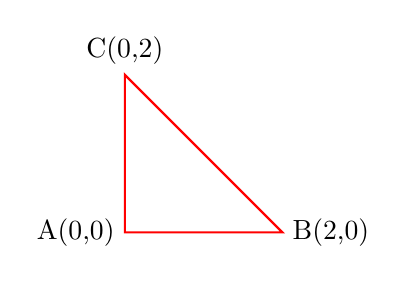
\begin{tikzpicture}
    \draw [color=red,thick] (0,0) node[anchor=east,text=black]{A(0,0)}--(2,0) node[right,text=black]{B(2,0)}--(0,2) node[above,text=black]{C(0,2)}--cycle;
\end{tikzpicture}
\vskip25pt

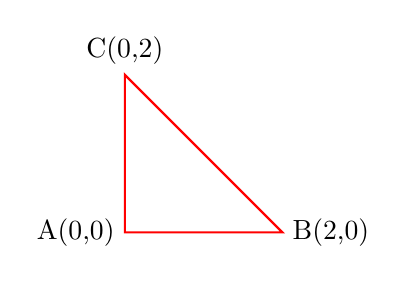
\begin{tikzpicture}
    \draw [color=red,thick] (0,0) node[anchor=east,text=black]{A(0,0)}--(2,0) node[right,text=black]{B(2,0)}--(0,2) node[above,text=black]{C(0,2)}--cycle;
\end{tikzpicture}
\vskip25pt

\end{document}